%% Q1
In \textbf{grounded theory} (Glaser \& Strauss, 1967) the \emph{constant comparative method} runs as a cycle. The researcher \textbf{collects data}, takes \textbf{field notes}, \textbf{codes} the data (open, axial and selective coding) and writes \textbf{memos}, comparing each new piece of data with earlier codes and categories until theoretical saturation is reached.
\why{(B) is Miles \& Huberman's interactive model of qualitative analysis; (C) mixes coding with narrative description; (D) describes generic thematic analysis.}

%% Q2
True experimental designs always have a \emph{control group} and random assignment. Quasi-experimental designs (e.g.\ the non-equivalent control group design) \emph{lack randomization} but still compare treated units with a control or comparison group. The common element, as per the official key, is the \textbf{control group}.
\why{Randomization is absent in quasi-experiments, and pre-testing is not used in every design (e.g.\ the post-test-only control group design).}

%% Q3
\begin{itemize}
\item Letters: G, J, M, P, S (+3) and T, R, P, N, L ($-2$) are both regular.
\item Numbers should follow $\times2+1, \times2+2, \times2+3, \times2+4$: $4\rightarrow\mathbf{9}\rightarrow20\rightarrow43\rightarrow90$.
\end{itemize}
The second term should be J\textbf{9}R, so \textbf{J10R} is wrong.

%% Q4
A cube cut into $3\times3\times3=27$ small cubes, with each face painted a different colour:
\begin{itemize}
\item corner cubes have 3 colours: \textbf{8};
\item edge (middle-of-edge) cubes have 2 colours: $12\times(3-2)=\mathbf{12}$;
\item face-centre cubes have 1 colour: 6; the central cube has none: 1.
\end{itemize}
Cubes with more than one colour $=8+12=\mathbf{20}$.

%% Q5
SWAYAM was developed by \textbf{MHRD (now MoE) and AICTE with the help of Microsoft}, not by UGC with Infosys. So statement (C) is not true. The other statements are correct: SWAYAM stands for \emph{Study Webs of Active-Learning for Young Aspiring Minds}, is India's MOOC platform, and was launched under Digital India.

%% Q6
\textbf{Kahoot}, \textbf{Socrative} and \textbf{Quizizz} are game-based, quiz-style learning and assessment platforms with points, leaderboards and timers.
\why{e-PG Pathshala is a UGC/INFLIBNET e-content repository for postgraduate subjects; Edmodo is a learning-management and social-classroom platform.}

%% Q7
$G/H$: G is the daughter of H. $H-I$: H is the mother of I. So I is a child of H, i.e.\ a sibling of G. The symbol ``$*$'' in $F*G$ is not defined in the code, and I's gender is not given, so ``Sister'' cannot be concluded. Mother and niece are clearly wrong. The official key gives \textbf{(D) No relation} (i.e.\ none of the definite relations offered can be established).

%% Q8 fig
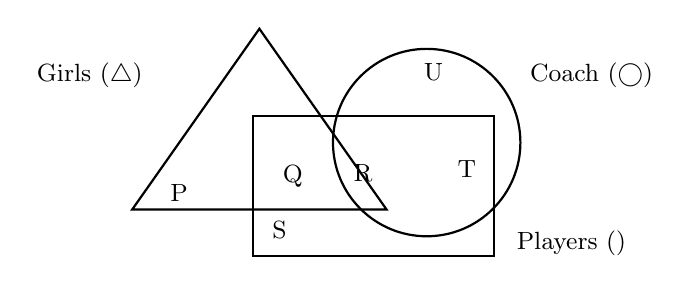
\begin{tikzpicture}[scale=0.85,font=\small]
\draw[thick] (-1.6,-0.5) -- (0.3,2.2) -- (2.2,-0.5) -- cycle;
\draw[thick] (0.2,-1.2) rectangle (3.8,0.9);
\draw[thick] (2.8,0.5) circle (1.4);
\node at (-0.9,-0.25) {P}; \node at (0.8,0) {Q}; \node at (1.85,0.05) {R}; \node at (0.6,-0.8) {S}; \node at (2.9,1.55) {U}; \node at (3.4,0.1) {T};
\node[left] at (-1.3,1.5) {Girls ($\triangle$)}; \node[right] at (4.2,1.5) {Coach ($\bigcirc$)}; \node[right] at (4.0,-1.0) {Players ($\square$)};
\end{tikzpicture}

%% Q8
Girls who are players but not coaches lie \textbf{inside the triangle and inside the square but outside the circle}. That region is \textbf{Q}.
\why{P = girls only; R = girls who are players \emph{and} coaches; S = players only (not girls).}

%% Q9
A good teacher is honest and a model learner: \textbf{appreciates the question and admits not knowing (5)}, \textbf{consults the library after class (4)} and \textbf{answers it the next day (2)}. Giving it as homework to hide ignorance (1) or sending the student away (3) is inappropriate. The answer is 2, 4 and 5.

%% Q10
In the \textbf{split-half method} one test is divided into two comparable halves (e.g.\ odd and even items), the two half-scores are correlated, and the result is stepped up with the Spearman--Brown formula $r_{tt}=\frac{2r_{hh}}{1+r_{hh}}$. It measures the \textbf{internal consistency of the whole test}.
\why{It needs a sufficiently large, even number of homogeneous items that can be split, and is unsuitable for speed tests.}

%% Q11 q
Match the List--I with List--II and choose the correct option given below.\\[2pt]
\begin{tabular}{@{}p{0.44\linewidth}p{0.5\linewidth}@{}}
\textbf{List--I} & \textbf{List--II}\\
1. National Institute of Educational Planning and Administration (NIEPA) & a. Deemed to be a University, 1964, under Section 3 of UGC Act, 1956\\
2. Tata Institute of Social Sciences (TISS) & b. A Central University and An Institution of National Importance\\
3. Mahatma Gandhi Antarrashtriya Hindi Vishwavidyalaya (MGAHV) & c. A Central University, established by an Act of Parliament, Act No.~3 of 1997\\
4. Visva-Bharati & d. Deemed to be University, 2006, under Section 3 of UGC Act, 1956\\
\end{tabular}

%% Q11 opts
1-b, 2-a, 3-c, 4-d
1-d, 2-a, 3-c, 4-b
1-b, 2-d, 3-c, 4-a
1-c, 2-b, 3-d, 4-a

%% Q11
\begin{itemize}
\item \textbf{NIEPA} (now NIEPA, New Delhi) became a deemed university in \textbf{2006}, so 1-d.
\item \textbf{TISS}, Mumbai (founded 1936) was declared deemed in \textbf{1964}, so 2-a.
\item \textbf{MGAHV}, Wardha was established by \textbf{Act No.~3 of 1997}, so 3-c.
\item \textbf{Visva-Bharati}, Santiniketan (founded by Tagore) is a central university and an \textbf{institution of national importance} (Visva-Bharati Act, 1951), so 4-b.
\end{itemize}

%% Q12
NEP~2020 proposes the \textbf{Higher Education Commission of India (HECI)} with four independent verticals:
\begin{enumerate}
\item \textbf{NHERC}, the National Higher Education Regulatory Council (regulation);
\item \textbf{NAC}, the National Accreditation Council (accreditation);
\item \textbf{HEGC}, the Higher Education Grants Council (funding);
\item \textbf{GEC}, the General Education Council (standard setting).
\end{enumerate}
A ``University Education Council'' is not one of them.

%% Q13
Using the given code: B$\rightarrow$R, R$\rightarrow$H, E$\rightarrow$P, A$\rightarrow$X, K$\rightarrow$B.
BREAK $\rightarrow$ \textbf{RHPXB}.

%% Q14
Until they meet, A and B together cover $PQ+QR+PR=2\times72=144$ km.
\[t=\frac{144}{17+19}=4\text{ h};\quad\text{B covers }19\times4=76\text{ km}=72+QR\ \Rightarrow\ QR=\mathbf{4\ km}\]

%% Q15
Mendeley is a \textbf{reference manager} (1-b); SPSS does \textbf{quantitative} analysis (2-a); Turnitin checks \textbf{plagiarism} (3-c); NVivo does \textbf{qualitative} analysis (4-d).

%% Q16
(a) $00111=7$, $01001=9$, $01011=11$: odd numbers, so next is $13=\mathbf{01101}$, not $011101$ ($=29$). Statement (a) is false.
(b) A byte is exactly 8 bits. Statement (b) is true. So \textbf{b only}.

%% Q17 q
Study the chart and answer the question. The pie chart given here represents the domestic expenditure of a family in percent. If the total monthly income of the family is Rs.~55,660/-, the annual savings in the form of PF would be (in nearest Rs.)

%% Q17 fig
\begin{tikzpicture}[scale=1]
\pie[radius=1.3,text=pin,color={brand!15,brand!35,brand!10,brand!45,brand!25,brand!5},font=\tiny]{9/Medical,13/PF,23/Food,18/House Rent,12/Entertain.,25/Child Edu.}
\end{tikzpicture}

%% Q17
Monthly PF $=13\%\times55{,}660=7{,}235.80$.
Annual PF $=7{,}235.80\times12=86{,}829.6\approx$ \textbf{Rs.~86,830}.

%% Q18 opts
\tikz[baseline=3mm,scale=0.45]{\draw[->](0,0)--(2.6,0);\draw[->](0,0)--(0,1.6);\draw[thick,brand](0,1)--(1.8,1);}
\tikz[baseline=3mm,scale=0.45]{\draw[->](0,0)--(2.6,0);\draw[->](0,0)--(0,1.6);\draw[thick,brand](0,0.8) .. controls (1.2,0.8) and (1.8,1) .. (2,1.5);}
\tikz[baseline=3mm,scale=0.45]{\draw[->](0,0)--(2.6,0);\draw[->](0,0)--(0,1.6);\draw[thick,brand](0,0)--(1.9,1.5);}
\tikz[baseline=3mm,scale=0.45]{\draw[->](0,0)--(2.6,0);\draw[->](0,0)--(0,1.6);\draw[thick,brand](0,0.6) .. controls (0.4,1.3) and (0.6,1.4) .. (0.9,0.9) .. controls (1.1,0.6) and (1.3,0.9) .. (1.6,0.95) -- (2.3,0.95);}

%% Q18
Plotting speed against time, excellent acceleration means the speed rises \textbf{quickly and steadily from rest}: a straight, steep line through the origin, as in graph (C).
\why{(A) shows constant speed (no acceleration); (B) starts with an almost flat curve (sluggish at first); (D) rises, falls and levels off.}

%% Q19
\textbf{Diagnostic evaluation} identifies the specific learning difficulties and their causes, so that remedial teaching can follow.
\why{Formative evaluation monitors progress during teaching; summative evaluation certifies achievement at the end.}

%% Q20
Slow learners need \textbf{tasks matched to their level and interests (2)}, \textbf{sufficient resources (4)} and \textbf{regular diagnosis and remediation (5)}. Treating them like everyone else or leaving them on their own (1, 3) neglects their needs. The answer is 2, 4 and 5.

%% Q21
\textbf{UNESCO} is the lead UN agency for \textbf{Education for Sustainable Development (ESD)}. It led the UN Decade of ESD (2005--2014), the Global Action Programme (2015--2019) and now the \emph{ESD for 2030} framework.

%% Q22
SDG~4 reads: ``\textbf{Ensure inclusive and equitable quality education and promote lifelong learning opportunities for all}'' by 2030.

%% Q23
Interval $k=600/30=20$. The selected numbers are $8, 28, 48, \ldots$, i.e.\ $8+20m$.
$88=8+80$ \checkmark, $368=8+360$ \checkmark, $428=8+420$ \checkmark, but $558-8=550$ is not a multiple of 20. So \textbf{558 is not selected}.

%% Q24 fig
\begin{tikzpicture}
\begin{axis}[ybar,width=10cm,height=4.4cm,bar width=11pt,ymin=0,ymax=5800,
  symbolic x coords={91-92,92-93,93-94,94-95,95-96,96-97,97-98,98-99},xtick=data,
  nodes near coords,every node near coord/.append style={font=\tiny},
  tick label style={font=\scriptsize},ylabel={\scriptsize million US\$},
  axis x line*=bottom,axis y line*=left]
\addplot[fill=brand!70,draw=brand] coordinates {(91-92,2640) (92-93,3720) (93-94,2520) (94-95,3360) (95-96,3120) (96-97,4320) (97-98,5040) (98-99,3120)};
\end{axis}
\end{tikzpicture}

%% Q24
\[\frac{\text{Reserves in 1997--98}}{\text{Reserves in 1994--95}}=\frac{5040}{3360}=\mathbf{1.5}\]

%% Q25
Poor listening, lack of trust and transparency, and cultural and language differences all hinder communication. A mere \textbf{difference in economic status} does not by itself prevent effective communication, so it is not a barrier in this list.

%% Q26
Effective classroom communication depends on the teacher's \textbf{sense of humour} (1), continuous \textbf{feedback} (2), appropriate \textbf{body language} (4) and a psychologically \textbf{safe environment} (5). Classroom cleanliness is a physical-hygiene factor, not a component of communication. The answer is 1, 2, 4, 5.

%% Q27
The \textbf{Doha Amendment} (COP18, Doha, December 2012) set up the \emph{second commitment period} of the Kyoto Protocol, from 2013 to 2020. (The first period ran 2008--2012.)
\why{The Paris Agreement (2015) is a separate treaty; the International Solar Alliance was launched by India and France in 2015; the Environment Protection Act is India's 1986 law.}

%% Q28
\textbf{Agenda 21}, adopted at the Rio Earth Summit (UNCED, 1992), is a comprehensive, non-binding plan of action to be taken \textbf{globally, nationally and locally} by the UN, governments and major groups in \textbf{every area in which humans impact the environment}. The ``21'' refers to the 21st century.

%% Q29
\textbf{Ex-post facto (causal-comparative) research} studies cause--effect relations after the fact. It starts from hypotheses about possible causes and \textbf{tests} them statistically.
\why{Historical, ethnographic and case-study research are mostly qualitative and exploratory; they generate hypotheses rather than test them.}

%% Q30
\textbf{Post-positivism} (Karl Popper and others) holds that all observation is theory-laden and \textbf{fallible}; objective reality exists but can be known only imperfectly and probabilistically. This critique of naive positivism opened the way to post-positivism.
\why{Options (A)--(C) restate \emph{positivist} ideas.}

%% Q31
If the price rises by $r\%$, then to keep the expenditure the same, consumption must fall by
\[\frac{r}{100+r}\times100=\frac{25}{125}\times100=\mathbf{20\%}\]

%% Q32
\textbf{Vyapti} is the invariable concomitance between the \emph{hetu} (middle term, \textbf{smoke}) and the \emph{sadhya} (major term, \textbf{fire}): ``wherever there is smoke there is fire''. So Vyapti is expressed by \textbf{fire and smoke}.

%% Q33
The \textbf{Kothari Commission} (1964--66) recommended spending \textbf{6\% of GDP} on education. The NPE 1986 (and its 1992 revision) and \textbf{NEP~2020} reiterated this target.

%% Q34
The \textbf{NCVET} (set up in 2018 under the Ministry of Skill Development) regulates the vocational education and training ecosystem. It recognises and regulates \emph{awarding bodies} and \emph{assessment agencies} and lays down standardised norms for quality. \textbf{Assessing and accrediting institutions of higher learning} is the job of NAAC, not NCVET.

%% Q35
In Nyaya philosophy, \textbf{Pratyaksha} (perception) is classified as \textbf{laukika} (ordinary perception through sense--object contact) and \textbf{alaukika} (extraordinary perception, namely samanya-lakshana, jnana-lakshana and yogaja).

%% Q36
Letters are removed alternately from the front (one letter) and from the end (two letters):
\begin{center}
SEQUENTIAL $\xrightarrow{-\text{S}}$ EQUENTIAL $\xrightarrow{-\text{AL}}$ EQUENTI $\xrightarrow{-\text{E}}$ \textbf{QUENTI} $\xrightarrow{-\text{TI}}$ QUEN
\end{center}

%% Q37
\textbf{Data mapping} matches fields from one database or dataset to another (1). It links sensitive data to the individual it belongs to (2), reduces errors and standardises data (3), and is central to data-privacy compliance such as the GDPR (4). Preparing graphs (5) is data \emph{visualisation}, not data mapping. The answer is 1, 2, 3, 4.

%% Q38
The cardinal philosophy of the NMEICT includes: no talent should go waste; all services through SAKSHAT should be free; freely available web material should be used rather than reinventing the wheel. \textbf{Rapid expansion of the optical-fibre network} is an infrastructure activity (connectivity component), not a cardinal philosophy.

%% Q39
Among the 17 SDGs: SDG~4 \textbf{Quality Education}, SDG~10 \textbf{Reduced Inequalities} and SDG~9 \textbf{Industry, Innovation and Infrastructure}.
\why{The goals are ``Life \emph{below} water'' (SDG~14) and ``Gender \emph{Equality}'' (SDG~5), not ``life beyond water'' or ``gender inequalities''.}

%% Q40
CFCs cause \textbf{ozone depletion} (1-b); SO$_2$ causes \textbf{acid rain} (2-a); lead harms the \textbf{nervous system} (3-d); CO$_2$ is the largest contributor to the \textbf{greenhouse effect} (4-c). The match is 1-b, 2-a, 3-d, 4-c.

%% Q41
Organisational barriers arise from the organisation itself: a complex structure, rigid or loose policies, poor facilities, and too many hierarchical levels. \textbf{Premature evaluation}, meaning judging a message before fully receiving it, is a \emph{psychological/personal} barrier.

%% Q42
Following Lasswell and Wright, the functions of mass communication are \textbf{surveillance} of the environment, \textbf{correlation} of society's responses (printed here as ``correction''), transmission of culture, and \textbf{entertainment}. Feedback is an element of the communication process, not a function of the mass media. The answer is 1, 2, 4.

%% Q43 ctx
\textbf{Directions for Q.~43 to 47:} Read the passage and answer the questions.\par\smallskip
International trade represents a significant share of Gross Domestic Product (GDP). While international trade has been present throughout much of history, its economic, social and political importance has been on the rise in recent times.

Industrialization, advances in technology, transportation, globalization, multi-national corporations, and outsourcing are having a major impact on the international trade. Increasing international trade is crucial to the continuance of globalization. International trade is, in principle, not different from domestic as the motivation and the behaviour of parties is across a boarder or not. International trade ``is typically more costly than domestic trade''. Another difference between domestic and international trade is that factors of production such as capital and labour are typically more mobile within a country than across countries.

%% Q43 q
Which of the following is not a factor of production?

%% Q43
The passage names \emph{capital and labour} as factors of production. In economics the factors are \textbf{land, labour, capital and entrepreneurship}. \textbf{Profit} is the \emph{reward} to the entrepreneur, not a factor.

%% Q44
``\textbf{Industrialization}, advances in technology, transportation, globalization, multi-national corporations, and outsourcing are having a major impact on the international trade.''

%% Q45
The passage says international trade is ``in principle, not different from domestic'' trade, but that it is more costly and involves factors that are less mobile across borders. Of the four options, the official key takes (D): international trade is the more \textbf{crucial} of the two, since it is ``crucial to the continuance of globalization'' and forms a significant share of GDP.

%% Q46
``Increasing international trade is \textbf{crucial to the continuance of globalization}.''

%% Q47
International trade ``is typically \textbf{more costly than domestic trade}'', because of transport, tariffs, currency exchange and so on.

%% Q48
Interpersonal communication is a \textbf{face-to-face exchange} (1-c); intrapersonal is \textbf{with oneself} (2-d); small group is \textbf{with a group sharing a common goal} (3-a); public communication is \textbf{strategic communication to convey ideas} to an audience (4-b). The match is 1-c, 2-d, 3-a, 4-b.

%% Q49
Appropriate statements: learning can occur without teaching, but teaching without learning is meaningless (1); teaching is giving and learning is receiving (2); teaching is the facilitation of learning (5).
Statement 3 has it backwards: teaching is usually called an \emph{art as well as a science}. Statement 4 is wrong because teaching is interactive and learning is often individual. The answer is 1, 2 and 5.

%% Q50
Effective teaching uses \textbf{appropriate teaching aids (2)}, \textbf{illustrations and examples (3)} and \textbf{two-way communication (5)}. Rote-learning the lesson (1) or writing everything on the board (4) makes teaching mechanical. The answer is 2, 3 and 5.
